%
% theory.tex
% Copyright (C) 2021 by Krish Kabra, <krish@kabra.com>.
%

\chapter{Theory}

\begin{figure}[t]
    \centering
    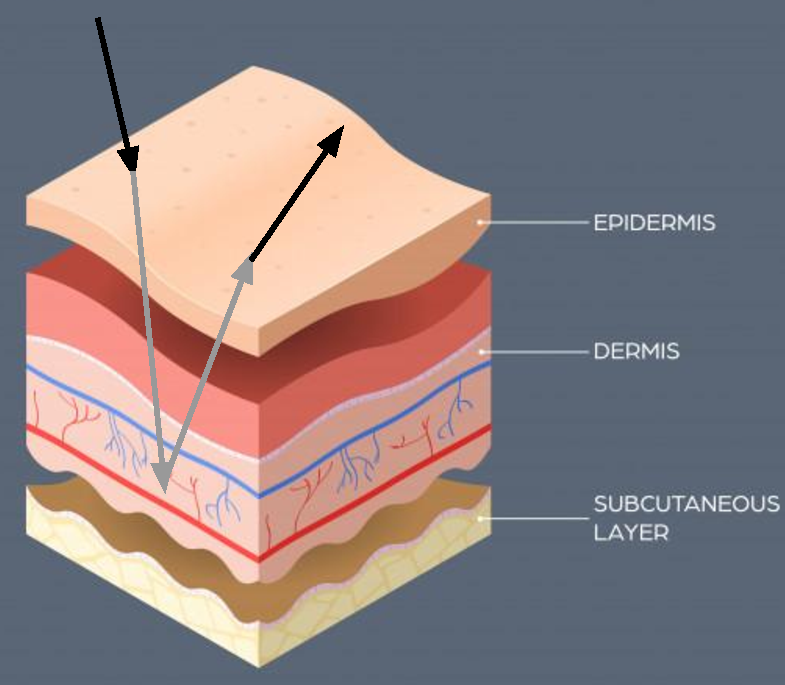
\includegraphics[height=3in]{include/fig_skin.pdf}
    \caption{\textbf{A two-layer skin model used in prior biorealistic rendering works is used to develop the light transport theory for R-PPG.} The incident light ray attenuates through the epidermis. Following dermal reflection and another epidermal attenuation, the resultant ray properties are dependent on human physiological quantities.}
    \label{fig:skin_model}
\end{figure}

Plethysmographic estimation methods are enabled through the sensing of blood perfusion in the face. Specifically, the presence of varying volumes of blood under the skin manifest as minute changes in reflection properties of the overall skin system, as viewed by a camera. It is by identifying these changes that relevant physiological properties may be estimated. 

In order to set up a novel light transport theory for R-PPG, we utilize existing biorealistic graphical rendering models~\cite{} and extend them for R-PPG signal generation. Figure~\ref{fig:skin_model} shows the skin model assumed for our computations, similar to~\cite{alotaibi_biophysical_2017}. Specifically, a two layer skin model is assumed. The incident light undergoes attenuation while passing through the epidermis, while it undergoes scattering driven reflection at the dermis. 

Using our light transport theory, we show that the signal strength reduces with increasing skin melanin content for all color channels, as intuitively expected. The decreasing signal strength leads us to an analysis of imaging noise, which is the major noise phenomenon at play in this case. Finally, with these mathematical insights, we conclude this section with a discussion on skin tone bias for r-PPG and propose solutions to improve performance on dark skin tone subjects.  

\section{Light Transport for R-PPG}

% \subsection{Epidermal Transmission}
We start with describing the epidermal transmission. Following the Beer-Lambert Law, 
\begin{equation} \label{eqn:T_epidermis}
    \mathbf{T_{epi}(\boldsymbol{\lambda})=e^{-\boldsymbol\mu_{a,epi}(\boldsymbol\lambda)}},
\end{equation}
Where $\mathbf{\boldsymbol\mu_{a,epi}(\boldsymbol\lambda)}$ is the absorption coefficient of the epidermis. Typically, this is modelled as a convex combination of skin tissue and melanin absorption,
\begin{equation} \label{eqn:mu_epidermis}
    \mathbf{\boldsymbol\mu_{a,epi}(\boldsymbol\lambda)=f_{mel}\boldsymbol\mu_{a,mel}(\boldsymbol\lambda)+(1-f_{mel})\boldsymbol\mu_{a,ski}(\boldsymbol\lambda)}.
\end{equation}

$\mathbf{\boldsymbol\mu_{a,ski}(\boldsymbol\lambda)}$, the skin tissue absorption coefficient, is a biological parameters which is known. $\mathbf{\boldsymbol\mu_{a,mel}(\boldsymbol\lambda)}$ may be defined as,
\begin{equation} \label{eqn:mu_melanin}
    \mathbf{\boldsymbol\mu_{a,mel}(\boldsymbol\lambda)=f_{eum}\boldsymbol\mu_{a,eum}(\boldsymbol\lambda)+(1-f_{eum})\boldsymbol\mu_{a,phm}(\boldsymbol\lambda)},
\end{equation}
Where ${\mathbf{\boldsymbol\mu_{a,eum}(\boldsymbol\lambda)}}$ is the absorption coefficient of eumelanin and $\mathbf{\boldsymbol\mu_{a,phm}(\boldsymbol\lambda)}$ is the absorption coefficient of pheomelanin, all biophysical known parameters. By combining Equations~\ref{eqn:T_epidermis}, \ref{eqn:mu_epidermis} and \ref{eqn:mu_melanin}, the epidermal transmission may be accurately modelled.

% \subsection{Dermal Reflection} 
We move towards describing the dermal reflection. This model follows the Kubelka-Munk theory for scattering-dependent reflection. Specifically, the fraction of reflected light, as a function of wavelength, is given by,
\begin{equation}
    \mathbf{R_{d}(\boldsymbol\lambda)=\frac{(1-\boldsymbol\beta(\boldsymbol\lambda))^2(e^{K(\boldsymbol\lambda)d_{der}}-e^{-K(\boldsymbol\lambda)d_{der}})}{(1+\boldsymbol\beta(\boldsymbol\lambda))^2e^{K(\boldsymbol\lambda)d_{der}}-(1-\boldsymbol\beta(\boldsymbol\lambda))^2e^{-K(\boldsymbol\lambda)d_{der}}}}
\end{equation}
Here, $\mathbf{\boldsymbol\beta(\boldsymbol\lambda)}$ and $\mathbf{K(\boldsymbol\lambda)}$ are deterministically related to $\mathbf{\boldsymbol\mu_{a,der}(\boldsymbol\lambda)}$ (dermal absorption coefficient) and $\mathbf{\boldsymbol\mu_{s,der}(\boldsymbol\lambda)}$ (reduced dermal scattering coefficient, known~\cite{}). Similar to previously, the dermal absorption coefficient and the blood absorption coefficient are understood as convex combinations shown below:
\begin{equation}
    \mathbf{\boldsymbol\mu_{a,der}(\boldsymbol\lambda)=f_{bld}\boldsymbol\mu_{a,bld}(\boldsymbol\lambda)+(1-f_{bld})\boldsymbol\mu_{a,ski}(\boldsymbol\lambda)}
\end{equation}
\begin{equation}
    \mathbf{\boldsymbol\mu_{a,bld}(\boldsymbol\lambda)=f_{oxy}\boldsymbol\mu_{oxy}(\boldsymbol\lambda)+(1-f_{oxy})\boldsymbol\mu_{dox}(\boldsymbol\lambda)}
\end{equation}
Here, various factors include blood reflection, skin baseline reflection, oxygenated blood reflection and deoxygenated blood reflection respectively.

% \subsection{Overall Reflection} 
Given the expressions for epidermal transmission and dermal reflection, the expression for overall reflection is given by,
\begin{equation}
    \mathbf{R(\boldsymbol\lambda) = T{^2}_{epi}.R_{d}(\boldsymbol\lambda)}.
\end{equation}

Then, the overall intensity captured in channel $\mathbf{c}$ of the camera is given by,
\begin{equation}
    \mathbf{I_c=\boldsymbol\int_{\boldsymbol\lambda}E(\boldsymbol\lambda)S_{c}(\boldsymbol\lambda)R(\boldsymbol\lambda)d\boldsymbol\lambda},
\end{equation}
Where $\mathbf{E(\boldsymbol\lambda)}$ is the source spectral distribution and $\mathbf{S_{c}(\boldsymbol\lambda)}$ is the camera spectral response for channel $\mathbf{c}$.

\section{R-PPG Signal Strength} 

\begin{figure}[t]
    \centering
    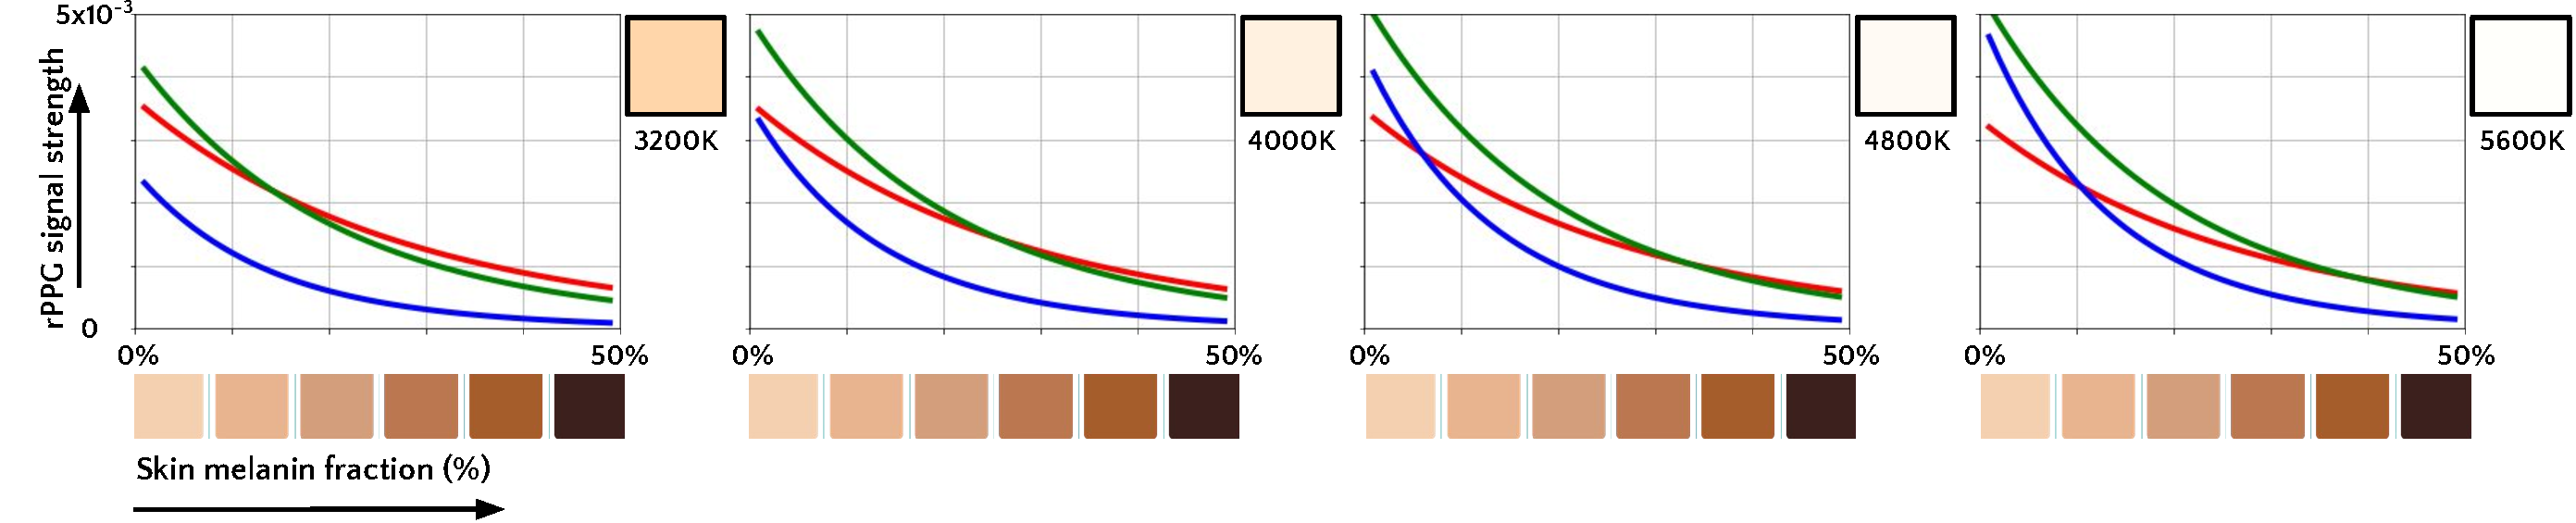
\includegraphics[width=\linewidth]{include/fig_strength.pdf}
    \caption{\textbf{The R-PPG signal strength is critically related to skin melanin fraction as well as scene lighting.} As opposed to previously accepted fact, the three channels may contain differing amounts of signal information, depending on regime of operation.}
    \label{fig:signal_strength}
\end{figure}

The R-PPG signal arises out of a variation in the blood volume fraction, $\mathbf{f_{bl}}$ under the skin. Our interest is in the signal strength across camera channels, $\boldsymbol\Sigma_{c}$, which can be defined as \textit{the maximum variation in the captured intensity}. Mathematically,
\begin{equation}
\begin{split}
    &\mathbf{\boldsymbol\Sigma_{c}=\boldsymbol\Delta I_c\boldsymbol\approx \Big|\frac{\boldsymbol\partial I_c}{\boldsymbol\partial f_{bl}}\Big|\cdot\boldsymbol\Delta f_{bl}}
\end{split}
\end{equation}
Since $\mathbf{R(\boldsymbol\lambda)}$ is the only term dependent on $\mathbf{f_{bl}}$,
\begin{equation}
\begin{split}
    &\mathbf{\boldsymbol\Sigma_{c}\boldsymbol\approx  \Big|\boldsymbol\int_{\boldsymbol\lambda}E(\boldsymbol\lambda)S_{c}(\boldsymbol\lambda)\frac{\boldsymbol\partial R}{\boldsymbol\partial f_{bl}}\Bigg|_{\overline{f_{bl}}} d\boldsymbol\lambda \Big| \cdot \boldsymbol\Delta f_{bl}},
\end{split}
\end{equation}
Where $\mathbf{\overline{f_{bl}}}$ is the average blood volume fraction, typically around $0.05$. This approximation holds true since $\mathbf{f_{bl}}$ only varies by a small amount, typically around $0.05$. 

This plethysmographic signal rides on top of the average skin tone color, given by
\begin{equation}
    \mathbf{\boldsymbol\Gamma_c=\boldsymbol\int_{\boldsymbol\lambda}E(\boldsymbol\lambda)S_{c}(\boldsymbol\lambda)R(\boldsymbol\lambda)\Big|_{\overline{f_{bl}}} d\boldsymbol\lambda}.
\end{equation}

Since, $\boldsymbol\Sigma_{c}$ and $\boldsymbol\Gamma_{c}$ are both dependent on $\mathbf{f_{mel}}$, as a result of the dependence of $\mathbf{R(\cdot)}$ on the same, we refer to these as $\mathbf{\boldsymbol\Sigma(f_{mel})}$ and $\mathbf{\boldsymbol\Gamma(f_{mel})}$ subsequently.

{\color{red} 
\begin{enumerate}
    \item Add parameter values used/the source paper for the same, for reproducability.
    \item Not clear what you mean by average camera response function. Also, where did we get the average response function from? We should cite our sources for reproducability. Same goes for light source characteristics.
\end{enumerate}
}

Figure~\ref{fig:signal_strength} shows the signal strength plots for the three camera color channels, across lighting conditions. We use average camera response functions $\mathbf{S_c(\boldsymbol\lambda)}$ to identify responsiveness of each of the channels to incident light. We also generate signal strength across common light source characteristics.  These plots provide incisive detail: the overall signal strength decays with increasing skin melanin fraction. Additionally, while previous works~\cite{verkruysse_remote_2008,haan_robust_2013,wang_algorithmic_2017} have empirically determined that the green channel holds maximum R-PPG signal information, we show for the first time that this in-fact heavily depends on melanin fraction. While the green channel is dominant for light skin tones, for darker skin tones, the channel-wise signal strength depends significantly on lighting conditions and skin tone.

\section{Effect of Imaging Noise on R-PPG}

\begin{figure}[t]
    \centering
    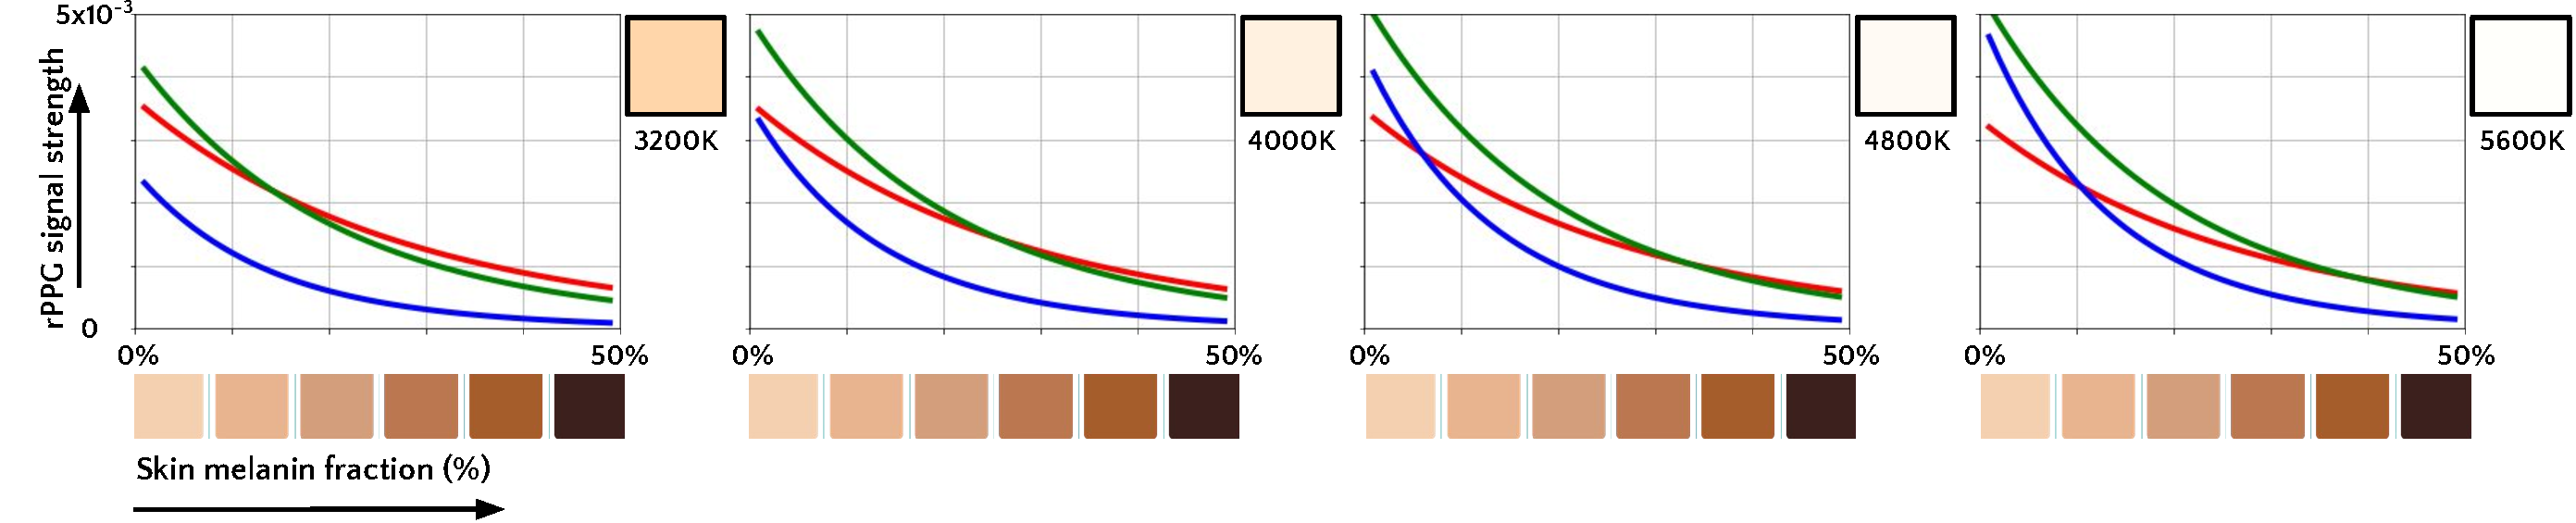
\includegraphics[width=\linewidth]{include/fig_strength.pdf}
    \caption{\textbf{FIGURE TO BE CHANGED!}}
    \label{fig:SNR_theory}
\end{figure}

The goal of this subsection is to understand the relationship between imaging noise and R-PPG algorithm estimation. Imaging noise refers to the inherent noise that arises due to the image capture process in a commercial camera. This arises due to various effects related to photon arrival processes, thermal noise in electronics and the quantization noise associated with digitally capturing images \cite{hasinoff_noise-optimal_2010}. For
pixels below the saturation level, the noise can be modelled as follows: 
\begin{equation} \label{eqn:imaging_noise_model}
    \sigma_{pixel}^2 = \frac{\Phi t}{g^2} + \frac{\sigma_{r}^2}{g^2} + \sigma_{q}^2
\end{equation}
where $\Phi$ is the radiant power of light collect, $t$ is the exposure time, $g$ is the sensor gain (a constant for a given image), and $\sigma_r$ and $\sigma_q$ are camera noie parameters (also constant). 

Using this noise model, we can the estimate the entire R-PPG signal to noise ratio (SNR) for a pixel of a particular intensity and color channel $c$ as follows:
\begin{equation} \label{eqn:SNR_rPPG}
    \mathbf{SNR_c} = \frac{\mathbf{\boldsymbol\Sigma_{c}}t}{\sqrt{\frac{\mathbf{\boldsymbol\Gamma_{c}}t}{g^2} + \frac{\sigma_{r}^2}{g^2} + \sigma_{q}^2}}
\end{equation}
Here, we assume that the radiant power of light collected $\Phi$ is equal to the average skin tone color. 

Figure~\ref{fig:SNR_theory} shows... These observations leads us to inferences

\section{Origins of Skin Tone Bias}

In recent years, the task

\cite{kadambi_achieving_2021}


\begin{enumerate}
    \item \textit{Imaging noise creates skin tone bias (and lighting bias)}

\end{enumerate}

\begin{figure}[t]
    \centering
    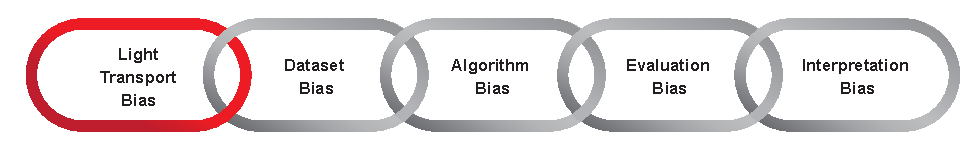
\includegraphics[width=\linewidth]{include/F_chain2.pdf}
    \caption{\textbf{The chain of biases in vision.}}
    \label{fig:chain_bias}
\end{figure}


% In recent years, there has been increasing interest in promoting the fairness of computer vision systems. A biased vision system for a task T, may operate differently when applied to certain subgroups of people or objects. To address this complex issue of fairness, colleagues have rightly pointed out factors that include dataset bias, algorithmic bias, or decision-making bias. However, there is another type of bias that is less discussed: the bias encountered by the laws of physics. Computer vision relies on light-sensing cameras - what if the physics of light involves bias? As one example, consider the task of face recognition with color cameras. We can immediately observe that a light-skinned face will fundamentally reflect more light (i.e. signal) than a dark-skinned face. More nuanced, however, are factors like the oiliness and texture of the face, which vary between males and females. These are forms of low-level bias. In this proposal, the PI lays the foundation for studying physical bias in a principled manner motivated by physics-based theory, experimental simulations, and ultimately the design of a novel colorless computational camera and health imagers that work consistently across skin tones. The work builds upon the PI’s deep expertise in low-level vision, imaging physics, and computational imaging. Further, the work lays a foundation for bringing physics into the realm of fair computer vision. 



% \section{Bias in R-PPG}

% \subsection{Algorithm Bias}

% \subsection{Dataset Bias}

% \subsection{Light Transport Bias}

